
\section{Location data and interactions}
\label{s:data-location}

Throughout this analysis, I use terminology of a productivity spillover occuring
from a group or average of \itx{peer} firms onto a \itx{target} firm.
The influence of the vector of all firms $j$ on the vector of all firms $i$
can be summarised in an $(n \times n)$ interactions matrix, $\mathbf W$.
\par
\todo{This can be explained better: in a table with 4 columns}
The interactions relationship is irreflexive. For groups it is transitive:
if firms A and B share a spatial group, such as a travel-to-work area (\itx{ttwa}),
first-half of a UK postocde (\itx{pc4}), or full postcode (\itx{pc8}),
then a firm C that is a peer of firm B must also be of firm A.
For continuous distance measures, this is non-transitive.
Firm B, a peer of firm A within its 5km radius, can clearly have its own peers
that are within its own 5km radius that are not shared with A.
Every firm is then its own overlapping group, or equivalently,
a sparse, rather than block diagonal, firm-to-firm matrix\footnote{
    I do actually impose a block diagonal structure for reasons of computation
    as explained subsequently
}.

\subsection{Location data limitations}
\label{ss:data-location-limits}
Fame only reports each company's last-known registered and trading address,
at the time of compilation of publication of its annual vintage\todo{cite}.
As a result, final location data is only available at the firm level.
We can interpret each firm as being static over the entire 20-year sample,
with no movers. This seems very unlikely \todo{expand}.
Instead, we must interpret the constructing address, and therefore firm-to-firm distance measures
as a signal of firm pairs' true distance polluted by movers.
This has 2 econometric consequences.
\par
Firstly, firm fixed effects in all spatial specifications become extremely important.
For all movers within the sample period, their firm location decision is endogenous to
the subsequent productivity spillovers they experience and exert,
for reasons discussed in Section \ref{s:literature} on New Economic Geography.
\todo{More on firm FEs}
There is no solution to this for moves occurring out-of-sample, for instance, just before 2009.
\par
Secondly, I acknowledge some attenuation to the productivity spillover estimate
Peer firms who were close to the target firm during the firm-year observation
who subsequently moved away within-sample will have an extreme distance recorded,
and so be excluded from tagged address groups and truncated distance calculations.
Peer firms who are recorded as close to the target firm as they subsequently moved to the location
\todo{More on direction of bias/positive selection?}

\subsection{Location group classification}

I first consider a model where each target has peers which share a spatial identifier,
meaning they belong to the same travel-to-work-area (\itx{ttwa}) using the 2011 definitions
\footnote{\todo{Review ONS bulletin on TTWAs data source and describe clearly}},
the first half of a UK postcode \itx{pc4},
and the full UK postcode \itx{pc8}.
\par
The structure of the weighting matrix $\mathbf W$ is key to identification.
$W$ is an $n\times n$ matrix of weights where each column $j$ denotes a weight $w_{ij}$
applied on the variable of peer firm $j$, summing across rows $i$
to reach a weighted aggregate regressor
with an estimated effect on target firm $i$.
\par
A first property of $W$ is that it its diagonal elements are all $0$:
a firm's TFP aggregate cannot be part of a weighted sum to an effect on its own TFP or GVA.
This is common to peer effets literature such as \cite{Moffitt2001}
and discussed in \cite{Bramoulle2009}.
\par
Group classifiers impose an otherwise block diagonal structure on $\mathbf W$.
The resulting $n\times n$ matrix has off-diagonal elements as
the number of group members $n_g-1$, which excludes the target firm $i$.
The structure is given below\footnote{
    Adapted from \cite{Bramoulle2009}
}:

\begin{align*}
    w_{ij}\in \mathbf W_g &=
        \begin{cases}
            0,              & \text{if}         \ i=j           \\
            \frac1{n_g-1},  & \text{else if}    \ (i,j)\in g    \\
            0,              & \text{otherwise}
        \end{cases}
    \\
    \mathbf \Gamma_{s_1} \in \mathbf W_g
    &=
    \{ i, j \in g \}, s_1: n_g
    \\
    \mathbf W_g
    &=
    \underset{(n\times n)}{
        \begin{pmatrix}
            \mathbf \Gamma_{s_1}    &   0                       &   \dots       \\
            0                       &   \mathbf \Gamma_{s_2}    &   \dots       \\
            \vdots                  &   \vdots                  &   \ddots
        \end{pmatrix}
    }
\end{align*}

\par\noindent
An example such matrix is $\mathbf W_{g^*}$, a $(7\times 7)$
set of interactions between firms which have group classifiers of size $s_1=4$ and $s_2=3$ only.

\begin{figure}[hbtp]
    \caption{Illustration of group matrix W}
    \label{fig:static-groups-W}
    \centering
    \par\noindent
    \begin{align*}
        \mathbf{W}_{g\sim \ref{fig:static-groups-W}}
        \begin{pmatrix}
            0           & \frac{1}{3} & \frac{1}{3} & \frac{1}{3} & 0           & 0           & 0           \\
            \frac{1}{3} & 0           & \frac{1}{3} & \frac{1}{3} & 0           & 0           & 0           \\
            \frac{1}{3} & \frac{1}{3} & 0           & \frac{1}{3} & 0           & 0           & 0           \\
            \frac{1}{3} & \frac{1}{3} & \frac{1}{3} & 0           & 0           & 0           & 0           \\
            0           & 0           & 0           & 0           & 0           & \frac{1}{2} & \frac{1}{2} \\
            0           & 0           & 0           & 0           & \frac{1}{2} & 0           & \frac{1}{2} \\
            0           & 0           & 0           & 0           & \frac{1}{2} & \frac{1}{2} & 0           
        \end{pmatrix}
    \end{align*}
    \begin{tablenotes}
        Weighting matrix $\mathbf W$ illustration for a network of 7 interacting firms in a group \itx{pc8}.
        Of these, firms 1-4 share their postcode, as do firms 5-7.
    \end{tablenotes}
\end{figure}

I can extend this to more complicated set of group rules.
I calculate non-overlapping group weights $\mathbf W_g$ to $\mathbf W_{g1}, \mathbf W_{g2}, \mathbf W_{g3}$ at once,
which represent the successive concentric rings of \itx(pc8) (core), \itx{pc4}, and \itx{ttwa}
The weighting rules for these multiple, non-overlapping groups is to zero the $i,j$ interaction in
$W_{gk}$ if a prior matrix in the series, $W_{gl},\ l<k$ has a non-zero entry in that cell.
I illustrate an example in Figure \ref{fig:static-groups-donut-matrices}.
These matrices are orthogonal.
\begin{align*}
        w_{ij}\in \mathbf{W}_{gk} &=
        \begin{cases}
            0,             & \text{if } i=j \\
            0,             & \text{if } w_{ij,l} \neq 0, \exists l<k \\
            \frac{1}{n_g-1}, & \text{else if } (i,j)\in g \\
            0,             & \text{otherwise}
        \end{cases}
\end{align*}

\begin{figure}[hbtp]
    \caption{Illustration of multiple, non-overlapping groups}
    \label{fig:static-groups-donut-matrices}
    \centering
    \par\noindent
    \begin{align*}
        \mathbf{W}_{g\sim \ref{fig:static-groups-donut-matrices}}
        &\sim
        \begingroup
        \setlength\arraycolsep{3.8pt}
        \begin{pmatrix}
            0 & \frac{1}{2} & \frac{1}{2} & 0 & 0 & 0 & 0 & 0 \\
            \frac{1}{2} & 0 & \frac{1}{2} & 0 & 0 & 0 & 0 & 0 \\
            \frac{1}{2} & \frac{1}{2} & 0 & 0 & 0 & 0 & 0 & 0 \\
            0 & 0 & 0 & 0 & 0 & 0 & 0 & 0 \\
            0 & 0 & 0 & 0 & 0 & 0 & 0 & 0 \\
            0 & 0 & 0 & 0 & 0 & 0 & 0 & 0 \\
            0 & 0 & 0 & 0 & 0 & 0 & 0 & 1 \\
            0 & 0 & 0 & 0 & 0 & 0 & 1 & 0
        \end{pmatrix}
        \begin{pmatrix}
            0 & 0 & 0 & \frac{1}{4} & \frac{1}{4} & 0 & 0 & 0 \\
            0 & 0 & 0 & \frac{1}{4} & \frac{1}{4} & 0 & 0 & 0 \\
            0 & 0 & 0 & \frac{1}{4} & \frac{1}{4} & 0 & 0 & 0 \\
            \frac{1}{4} & \frac{1}{4} & \frac{1}{4} & 0 & \frac{1}{4} & 0 & 0 & 0 \\
            \frac{1}{4} & \frac{1}{4} & \frac{1}{4} & \frac{1}{4} & 0 & 0 & 0 & 0 \\
            0 & 0 & 0 & 0 & 0 & 0 & \frac{1}{2} & \frac{1}{2} \\
            0 & 0 & 0 & 0 & 0 & \frac{1}{2} & 0 & 0 \\
            0 & 0 & 0 & 0 & 0 & \frac{1}{2} & 0 & 0
        \end{pmatrix}
        \begin{pmatrix}
            0 & 0 & 0 & 0 & 0 & \frac{1}{8} & \frac{1}{8} & \frac{1}{8} \\
            0 & 0 & 0 & 0 & 0 & \frac{1}{8} & \frac{1}{8} & \frac{1}{8} \\
            0 & 0 & 0 & 0 & 0 & \frac{1}{8} & \frac{1}{8} & \frac{1}{8} \\
            0 & 0 & 0 & 0 & 0 & \frac{1}{8} & \frac{1}{8} & \frac{1}{8} \\
            0 & 0 & 0 & 0 & 0 & \frac{1}{8} & \frac{1}{8} & \frac{1}{8} \\
            \frac{1}{8} & \frac{1}{8} & \frac{1}{8} & \frac{1}{8} & \frac{1}{8} & 0 & 0 & 0 \\
            \frac{1}{8} & \frac{1}{8} & \frac{1}{8} & \frac{1}{8} & \frac{1}{8} & 0 & 0 & 0 \\
            \frac{1}{8} & \frac{1}{8} & \frac{1}{8} & \frac{1}{8} & \frac{1}{8} & 0 & 0 & 0
        \end{pmatrix}
        \endgroup
    \end{align*}
    \begin{tablenotes}
        Non-overlapping group illustration for a network of 8 interacting firms in a \itx{ttwa}.
        Of these, firms 1-5 share the first half of a postcode - are in a \itx{pc4} group, as are firms 6-8.
        Within those, firms 1-3 share a full postcode, as do firms 7-8. Firms 4-6 are isolated in their \itx{pc8} groups.
    \end{tablenotes}
\end{figure}

Firms have been labelled using their location features to symmetric, transitive,
non-overlapping groups by \itx{ttwa} (largest) to \itx{lat\_lon5} (smallest),
with the latter meaning two firm entries shared a latitude-longitude identifier
to 5 decimal places.
Reviewing the summary statistics, I opted for full postcodes, \itx{pc8}
as the group identifier for initial 1-group models in Table \ref{tab:lmm-pc8}.
This was mostly driven by full data availability, and the consistency of postcode definitions
with the larger group $pc4$. Deriving a subgroup by latitude-longitude match
within the postcode seemed fruitless, as in many cases it would identify the exact same firms,
a move from the average number of peers from 3.1 to 2.9,
and was a similar number of groups, with non-coheisve definitions.
\wraptable
    {Summary statistics across location groups}
    {./figures/3_tab_summary_w_groups}
    {}

\subsection{\todo{Location distance calculations}}
\label{ss:data-distance}

\begin{figure}[hbtp]
    \caption{Histogram of distances between any target-firm pairing}
    \label{fig:hist-distances-20km}
    \centering
    \graphicspath{ {../../calculations/output/}}
    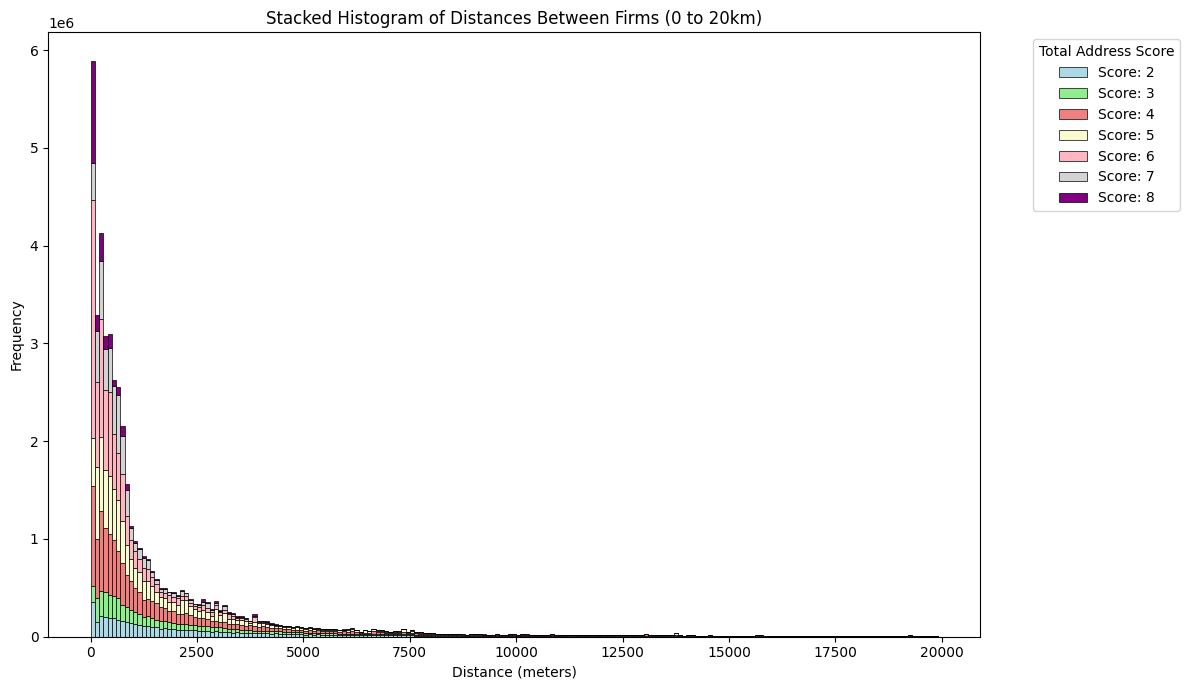
\includegraphics[width=\textwidth]{histogram_distances_20km.png}
    \begin{tablenotes}
        Plotted into bins of 100m distance measures. Using the \itx{d1} distance measure,
        which is hard-bounded that no firm can have a firm-peer spillover relation past a \itx{ttwa} boundary,
        truncated at 20km.
        Colours indicate differing levels of data quality for addresses within Fame.
        \\
        \todo{This must be an old chart, I think we truncated at 5km in the end.
        Also, to produce without colours as this adds confusion}
    \end{tablenotes}
\end{figure}

\subsection{Iterative weighting applications}
\label{ss:data-matrix-weights}

\wraptable
    {Variable names from transforming $\mathbf y_t$ and $\mathbf x_t$ regressors via weighting matrix $\mathbf W$} 
    {../../calculations/output/3_group_w_prefixes}
    {Total: 51 new variables to be created, for a total of 53 columns in a linked table.}

Intuitively, I take the product of these weighting matrices $\mathbf W$ to the aggregate variables vectors
\itx{gva1}, capital \itx{total\_assets}, and labour \itx{employees}.
As will be shown in \fullref{s:models-static}, the procedure to generate valid instrumental variables
also requires me to apply multiples of this transformation matrix,
exponents $\mathbf W^2, \mathbf W^3, \mathbf W^4$, and for interacting group matrices,
$\mathbf W_{g1}\mathbf W_{g2}, \mathbf W_{g2}\mathbf W_{g3}$ and so on to the aggregates.
\par
As a data procedure, I calculate these for my 3 aggregate variable vectors of interest.
As given below in Table \ref{tab:w_prefixes}, this requires a total of 51 compound weighting matrices,
or columns of a database, to be calculated and generated.
Of course, these column vectors each contain a stacked \itx{firm} ($i$)-\itx{year} ($t$)
observation, giving an additional matrix of over 1 million entries.

Matrix products, including taking high indices, of the interactions between 1,52,379 firms
is not computationally difficult, especially with sophisticated algorithms to handle $W$'s block diagonal structure.
However, storing the calculation in temporary memory is beyond
the capacity of any standard machine available as a research tool.
\par
Instead, I use a computational approach that avoids calculating the $\mathbf W^2, W^3...$ matrix
separately, but rather iteratively applies the last pre-multipled matrix to the aggregate variable,
and then pre-multiplies the next matrix along to the result.
Using memory-efficient \itx{duckdb}, the procedure is as follows:
\todo{itemize}

\subsection{Evaluating the linear independence of W matrices}

As will be discussed more heavily in the theory of \ref{ss:static-identification},
the key condition of these $\mathbf W$ matrices that will permit valid instrumentation of endogenous variables
is to check the linear independence of $\mathbb I, \mathbf W, \mathbf W^2$, and later $\mathbf W^3$.
I can trivially say this is true, meeting the alternative sufficient conditions in \ref{tab:bdf_identification}
of $\geq 3$ group sizes for the group $\mathbf W$ matrices.
\todo{Histogram of group sizes?}
\par
My distance-decay weights, $\mathbf W_{d1}, \mathbf W_{d2}, \mathbf W_{d3}$
meet the strong alternative $s_d\geq 3$ condition, where $s_d$ is the \itx{diameter} of the network,
the maximal number of links connecting any target $i$ with another firm through a series of peers $j, k, \dots$.
In the analysis of this set of firms with distance radius limits,
the \itx{diameter} is large, potentially spanning the full spatial diameter of a \itx{ttwa}.
It is this mechanism design provides another justification, alongside computation,
for limiting the max length of a target-firm peer relation to 5km:
it vastly increases the probability of `overlapping groups', i.e. a high diameter network within a `itx{ttwa}'.
The overlapping group network structure lends itself nicely to illustrations.
Figure \ref{fig:map-nolg-manc} selects a random firm $i$ from my sample,
which happens to be in Stockport, Greater Manchester, and draws the distances used to calculate metric $d1$
between this target and its peers. In typical network diagram fashion, a network with a considerable \itx{diameter}
is created by taking a subset of $i$'s peers, then successively a set of their peers, then successively some of those
and so on. 4 iterations in this diagram fails to clearly hit the \itx{ittwa} boundary,
on the south side, with more argument for this behaviour on the north side
where peer nodes randomly selected may be starting to bunch at an `invisible' border of the \itx{ttwa} boundary.

\begin{figure}[hbtp]
    \caption{Illustration (2) of overlapping groups from a target firm to its whole network through successive peers}
    \label{fig:map-nolg-manc}
    \centering
    \graphicspath{ {../../calculations/output/}}
    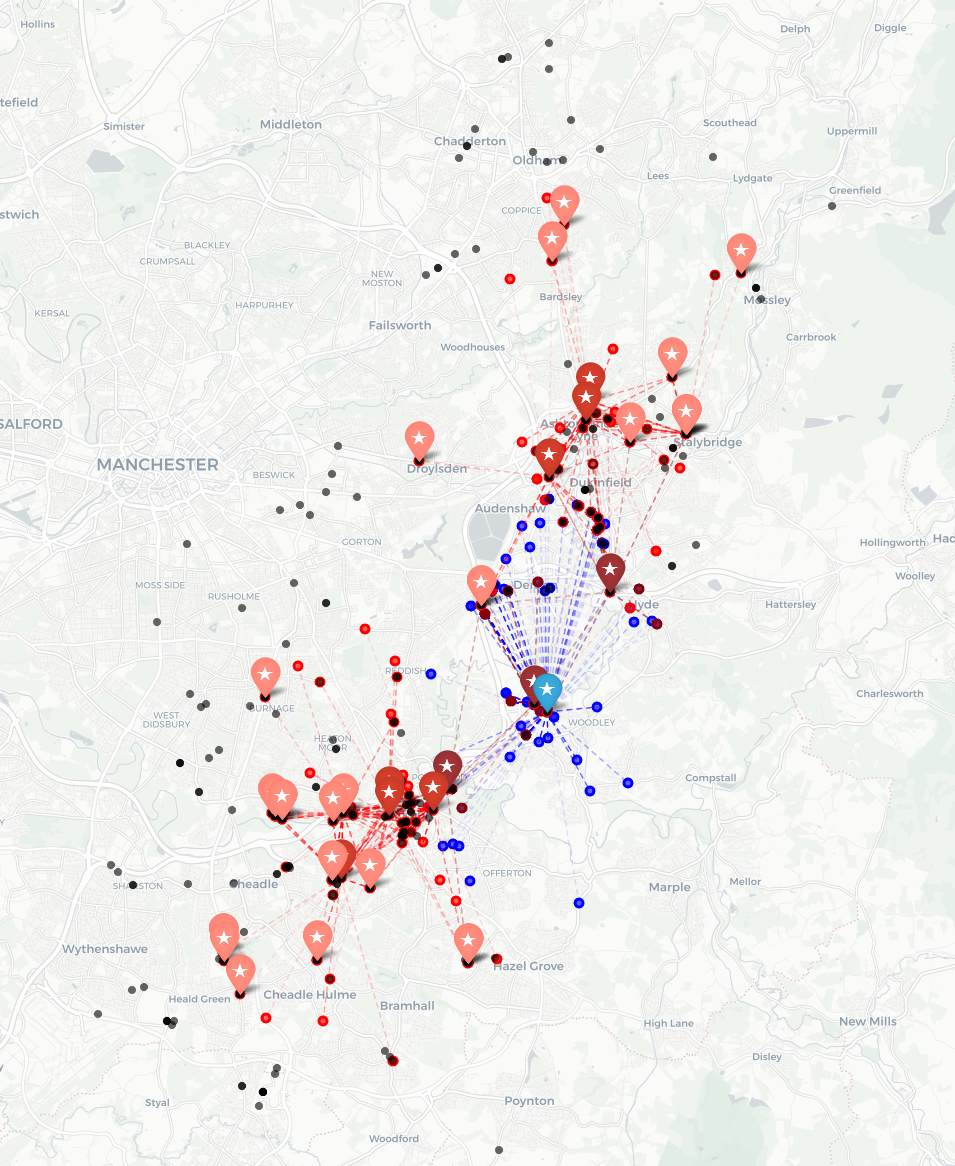
\includegraphics[width=\textwidth]{distance_peers_nolg3.png}
    \begin{tablenotes}
        (blue pin): target firm $i$ with a full set of its (blue dot) peers $j$,
        distances $d_1$ metric drawn in.
        \newline
        (dark red pins): sample (limit 5) of $j$ peers, then calculated as their own targets
        \newline
        (red pins): sample (limit 5) of $k$ peers of firms $j$, some of which are also shared as a peer of $i$.
        \newline
        (light red pins): sample (limit 5) of $m$ peers of firms $k$, few of which are also shared as a peer of $i$.
        \newline
        (light red dots): set of $n$ peers of firms $m$, few of these are peers of $i,j$,
        probabilistically creating a network diameter of $s_d\geq 3$.
        Plotting software from \cite{Folium2012}. Map tiles from \cite{CARTO2026}.
    \end{tablenotes}
\end{figure}

\par
As additional credibility, I discuss strategies for evaluating the linear independence
of $\mathbb I, \mathbf W, \mathbf W^2$ \todo{\dots}